\documentclass[11pt,a4paper,twoside,pdf]{article}

% Encoding and typography
\usepackage[T1]{fontenc}
\usepackage[utf8]{inputenc}
\usepackage{mathpazo}
\usepackage{braket}

% Mathematics
\usepackage{amsmath, amssymb, amsfonts}
\usepackage{bm}
\usepackage[mathscr]{euscript}

% Figures
\usepackage{graphicx}
\usepackage{float}
\usepackage{subcaption}

% Tables and utilities
\usepackage{multirow}
\usepackage{rotating}
\usepackage{array}
\usepackage{booktabs}
\usepackage{xspace}

% Extra symbols
\usepackage{eurosym}
\usepackage{bbding}
\usepackage{pifont}

% Others
\usepackage{soul}
\usepackage{color}
\usepackage{latexsym}
\usepackage{xtab}

% Hyperlinks
\usepackage[colorlinks=true,urlcolor=blue,linkcolor=blue,citecolor=blue]{hyperref}

% Equation numbering
\numberwithin{equation}{section}

% Margins
\usepackage[top=2.88cm,bottom=2.97cm,left=2.95cm,right=2.95cm]{geometry}

% Language
\usepackage[english]{babel}

% Headers
\usepackage{fancyhdr}


% Theorems
\newtheorem{theorem}{Theorem}[section]
\newtheorem{corollary}{Corollary}[theorem]
\newtheorem{lemma}[theorem]{Lemma}


%EXTRAS---------------------------------------------------------------------------------------------------
\usepackage{forest}
\usepackage{tikz}
\usepackage{tikz-qtree}

\usepackage{listings}
\usepackage{xcolor}

\definecolor{codegreen}{rgb}{0,0.6,0}
\definecolor{codegray}{rgb}{0.5,0.5,0.5}
\definecolor{codepurple}{rgb}{0.58,0,0.82}
\definecolor{backcolour}{rgb}{0.95,0.95,0.92}

\lstdefinestyle{mystyle}{
    backgroundcolor=\color{backcolour},
    commentstyle=\color{codegreen},
    keywordstyle=\color{magenta},
    stringstyle=\color{codepurple},
    basicstyle=\ttfamily\footnotesize,
    breaklines=true,
    captionpos=b,
    keepspaces=true,
    numbers=none,
    showspaces=false,
    showstringspaces=false,
    showtabs=false,
    tabsize=2
}

\lstset{style=mystyle}


% Custom commands
\newcommand{\dis}{\displaystyle}

\linespread{1.05}

\begin{document}

% Cover %%%%%%%%%%%%%%%%%%%%%%%%%%%%%%%%%%%%%%%%%%%%%%%%%%%%%%%%%%%%%%%%%%%%%%

\pagestyle{empty}

\noindent
\begin{tabular}{r}

\includegraphics[width=8.8cm]{escudoUGRmonocromo.png} \\[-1.8ex]
\hspace{31mm}\vspace{-8mm}
\begin{tabular}{c}
\hline\\[-1ex]\hskip-2mm
{\bf Faculty of Sciences}\hspace{18mm}
\end{tabular}
\end{tabular}

\large
\vspace{10mm}
\hspace{25mm}
\begin{tabular}{l}
M.Sc.\ in Physics: Radiation, Nanotechnology, \\ Particles and Astrophysics \\
\end{tabular}


\vspace{5mm}
\hspace{25mm}
\begin{tabular}{l}
Mathematical and Numerical Complements
\\[1.5ex]
\LARGE\bf Discrete and Fast \\
\LARGE\bf Fourier Transform
\end{tabular}
%

\hspace{2mm}
\begin{tabular}{l}
By:
\\
{\bf A. S. Amari Rabah}\\
\end{tabular}


\begin{abstract}

We study the discrete Fourier transform (DFT) and its efficient implementation through the Fast Fourier Transform (FFT) algorithm by means of two self-contained implementations in their recursive and iterative forms. The numerical results are compared against analytical solutions and the \texttt{np.fft()} routine of the NumPy library for a collection of representative functions. The fundamental properties of the Fourier transform are then verified numerically. Finally, we formulate the application of the FFT in quantum mechanics and use it to solve the Schr\"odinger equation by spectral methods, with an explicit example on the quantum harmonic oscillator.

\end{abstract}

% Indice %%%%%%%%%%%%%%%%%%%%%%%%%%%%%%%%%%%%%%%%%%%%%%%%%%%%%%%%%%%%%%%%%%%%%%%

\tableofcontents

% Text %%%%%%%%%%%%%%%%%%%%%%%%%%%%%%%%%%%%%%%%%%%%%%%%%%%%%%%%%%%%%%%%%%%%%%%%

\pagestyle{fancy}
\fancyhead[RO,LE]{\leftmark}
\fancyhead[LO,RE]{\thepage}
\fancyfoot{}



\newpage


\section{Introduction}
\label{intro}


The direct discrete Fourier transform (DFT) is defined as \cite{angulo2012variable}

\begin{equation}
    X[k] = \sum_{n=0}^{N-1} x[n] e^{-j\frac{2\pi}{N}kn},
\tag{1}
\label{DDFT}
\end{equation}

and its inverse

$$
    x[n] = \frac1N\sum_{k=0}^{N-1} X[k] e^{j\frac{2\pi}{N}kn},
$$


with $x[n], n = 0, 1, \cdots, N-1$ and $k = 0, 1, \cdots, N-1$. In matrix form

$$
    X = W_N x,
$$

where the matrix $W_N$ has entries $W^{k,n}_N = e^{-j\frac{2\pi}{N}kn}$. Computing the Fourier transform of a signal directly therefore costs $\mathcal{O}(N^2)$. The Fast Fourier Transform (FFT) reduces this to $\mathcal{O}(N\log N)$ \cite{brigham1988fast}.

\subsection{Fast Fourier Transform}


The FFT splits the vector $x$ into its even-indexed and odd-indexed components recursively, until reaching the base case $N=1$ where $\mathrm{FFT}(a) = a$. Hence this fast version of the algorithm requires the length of the vector to be a power of two ($N = 2^m$).

Splitting the sum \ref{DDFT} into even and odd terms yields

$$
    X[k] = \sum_{n=0}^{N-1} x[n] e^{-j\frac{2\pi}{N}kn}
    = \sum x[2n] e^{-j2\pi k (2n) / N} +
    \sum x[2n+1] e^{-j2\pi k (2n+1) / N}
$$

$$
    = \sum x_{\text{even}}[n] e^{-j2\pi kn / (N/2)} +
    e^{-j2\pi k/N} \sum x_{\text{odd}}[n] e^{-j2\pi k n / (N/2)}.
$$

Defining

$$
    P[k] = \mathrm{DFT}[x_{\text{even}}], \qquad I[k] = \mathrm{DFT}[x_{\text{odd}}],
$$


one obtains

$$
    X[k]=P[k]+W^k_N I[k]
$$

where $W_N^k = e^{-j2\pi k/N}$. Only half of the spectrum needs to be computed, since $e^{-j2\pi (k+N/2)n/N} = e^{-j2\pi kn/N} e^{-j2\pi (N/2)n/N}$ and $e^{-j2\pi (N/2)n/N} = e^{-j\pi n} = (-1)^n$, so

$$
    X[k + N/2] = P[k] - W^k_N I[k].
$$


Applying this same procedure to the transforms $P[k]$ and $I[k]$ of size $N/2$, and so on recursively, one eventually reaches $N=1$, where the DFT is trivial.

At each recursion level there are $N$ operations, and the number of levels is $\log_2 N$, so the total cost is $\mathcal{O}(N\log N)$.

We now present two different implementations of the FFT.



\subsubsection{Recursive method}


The recursive method calls itself repeatedly (combining even and odd halves) until the trivial base case is reached. It is very simple to implement, but requires allocating new vectors at each subdivision, which increases memory usage. Using NumPy ($ver.$ $1.26.4$) \cite{harris2020array} and Python ($ver.$ $3.12.10$) the function reads\\



\begin{lstlisting}[language=Python, caption = Recursive FFT implementation.]
import numpy as np

def fft_rec(x, inverse=False):

    x = np.asarray(x, dtype=complex)
    N = x.shape[0]

    if N == 1:
        return x.copy()

    if N % 2 != 0:
        raise ValueError("N must be a power of 2")

    sign = 1 if inverse else -1

    # Recursion
    X_even = fft_rec(x[::2], inverse)
    X_odd  = fft_rec(x[1::2], inverse)

    X = np.zeros(N, dtype=complex)

    # Twiddle factors (W_{k+1} = W_k * W_1)
    W1 = np.exp(sign * 2j * np.pi / N)
    W = 1.0 + 0j

    for k in range(N // 2):

        t = W * X_odd[k]

        X[k]          = X_even[k] + t
        X[k + N // 2] = X_even[k] - t

        W *= W1

    if inverse:
        X /= 2

    return X
\end{lstlisting}




\subsubsection{Iterative method}


The iterative method operates on the vector $x$ in place and hence does not suffer from the memory overhead of the recursive version. The FFT requires sorting the input by repeatedly splitting odd and even indices, which can be done efficiently via \textit{bit-reversal}.

At the first level the FFT selects even and odd components, which in binary means picking all entries whose last bit is 0 for the evens and 1 for the odds. At the next level the last bit is dropped and one splits again by the next-to-last bit, and so on until the final level. For a vector of length $N = 8$ the algorithm gives

\begin{itemize}
    \item Level 0: \qquad $(x_0, x_1, x_2, x_3, x_4, x_5, x_6, x_7)$
    \item Level 1: \qquad $(x_0, x_2, x_4, x_6 \mid x_1, x_3, x_5, x_7)$
    \item Level 2: \qquad $(x_0, x_4 \mid x_2, x_6 \mid x_1, x_5 \mid x_3, x_7)$
    \item Level 3: \qquad $(x_0 \mid x_4 \mid x_2 \mid x_6 \mid x_1 \mid x_5 \mid x_3 \mid x_7)$
\end{itemize}

In other words, the entry at position $b_{N-1}\cdots b_{1}b_{0}$ ends up at position $b_0 b_{1}\cdots b_{N-1}$: its bit order is reversed. Once the bit-reversed vector is obtained, the algorithm reconstructs the transform by progressively combining values with the twiddle factors

\[
W_8^k = e^{-2\pi i k/8}.
\]


The reconstruction proceeds in three stages ($2^3 = 8$).

In stage 1 the data are grouped in pairs and size-2 transforms are computed

\[
\begin{aligned}
a_0 &= x_0 + x_4, & b_0 &= x_0 - x_4,\\
a_1 &= x_2 + x_6, & b_1 &= x_2 - x_6,\\
a_2 &= x_1 + x_5, & b_2 &= x_1 - x_5,\\
a_3 &= x_3 + x_7, & b_3 &= x_3 - x_7.
\end{aligned}
\]

yielding

\[
(a_0,b_0,a_1,b_1,a_2,b_2,a_3,b_3).
\]

In stage 2 four-element blocks are combined using the factors

\[
W_4^k = e^{-2\pi i k/4}, \qquad k=0,1.
\]

For the first block

\[
\begin{aligned}
c_0 &= a_0 + W_4^0 a_1 = a_0 + a_1,\\
c_1 &= b_0 + W_4^1 b_1 = b_0 - i b_1,\\
c_2 &= a_0 - W_4^0 a_1 = a_0 - a_1,\\
c_3 &= b_0 - W_4^1 b_1 = b_0 + i b_1,
\end{aligned}
\]

and analogously for the second

\[
\begin{aligned}
c_4 &= a_2 + a_3,\\
c_5 &= b_2 - i b_3,\\
c_6 &= a_2 - a_3,\\
c_7 &= b_2 + i b_3.
\end{aligned}
\]

yielding

\[
(c_0,c_1,c_2,c_3,c_4,c_5,c_6,c_7).
\]


Finally all coefficients are combined with

\[
W_8^k = e^{-2\pi i k/8}, \qquad k=0,1,2,3,
\]

giving

\[
\begin{aligned}
X_0 &= c_0 + W_8^0 c_4, &
X_4 &= c_0 - W_8^0 c_4,\\
X_1 &= c_1 + W_8^1 c_5, &
X_5 &= c_1 - W_8^1 c_5,\\
X_2 &= c_2 + W_8^2 c_6, &
X_6 &= c_2 - W_8^2 c_6,\\
X_3 &= c_3 + W_8^3 c_7, &
X_7 &= c_3 - W_8^3 c_7.
\end{aligned}
\]

The final vector

\[
(X_0,X_1,X_2,X_3,X_4,X_5,X_6,X_7)
\]

coincides with the discrete Fourier transform of the original input.


Each stage doubles the size of the previously computed sub-transforms by introducing the phase factors $W_N^k$. After $\log_2 N$ stages the full DFT is obtained at cost $\mathcal{O}(N\log N)$. The following snippet implements the iterative FFT for arbitrary power-of-two $N$\\



\begin{lstlisting}[language=Python, caption = Iterative FFT implementation.]
import numpy as np

def fft_it(x, inverse=False):

    x = np.asarray(x, dtype=complex).copy()
    N = x.shape[0]

    if (N & (N - 1)) != 0:
        raise ValueError("N must be a power of 2")

    # -------------------------
    # 1) BIT REVERSAL
    # -------------------------

    nbits = int(np.log2(N))

    def bit_reverse(n, bits):
        r = 0
        for _ in range(bits):
            r = (r << 1) | (n & 1)
            n >>= 1
        return r

    for i in range(N):
        j = bit_reverse(i, nbits)
        if j > i:
            x[i], x[j] = x[j], x[i]

    # -------------------------
    # 2) STAGES
    # -------------------------

    sign = 1 if inverse else -1

    m = 2
    while m <= N:

        half = m // 2
        Wm = np.exp(sign * 2j * np.pi / m)

        for k in range(0, N, m):

            W = 1.0 + 0j

            for j in range(half):

                t = W * x[k + j + half]
                u = x[k + j]

                x[k + j]        = u + t
                x[k + j + half] = u - t

                W *= Wm

        m *= 2

    # -------------------------
    # 3) IFFT NORMALISATION
    # -------------------------

    if inverse:
        x /= N

    return x
\end{lstlisting}




\section{Particular cases}


In this section we evaluate the Fourier transform of several typical functions using the implementations above and compare them against the NumPy \texttt{np.fft()} routine. The error is measured as the $L^2$ norm of the difference between analytical and numerical solutions.

In all cases excellent agreement with the analytical solution is found, and the error stays at the level of $10^{-10}$ for both iterative and recursive implementations.


\subsection{Sines and cosines}

\begin{figure}[H]
    \centering
    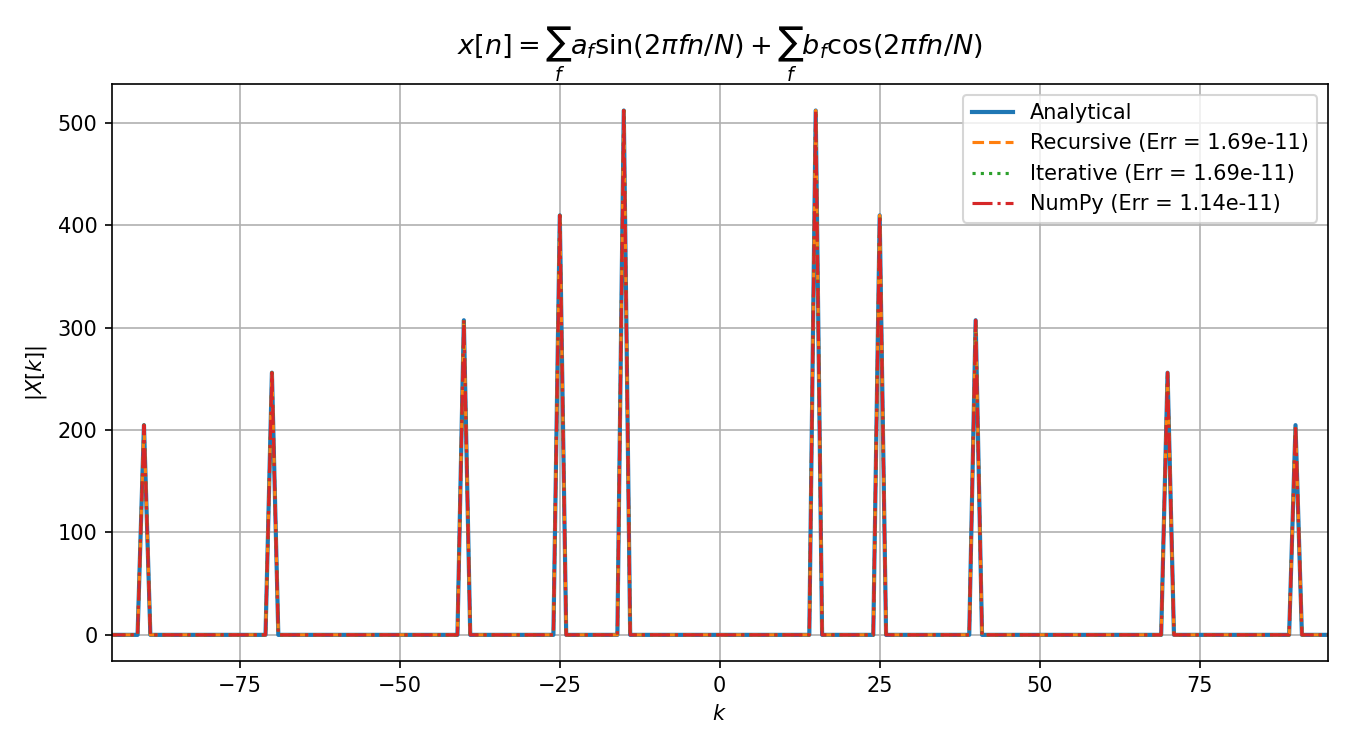
\includegraphics[width=1\linewidth]{../figures/sine_cosine.png}
    \caption{Comparison between the DFT computed with our recursive and iterative codes, the NumPy routine \texttt{np.fft()}, and the analytical solution for a sum of sines and cosines. $N = 1024$ points are used. The error is the $L^2$ norm.}
    \label{senoycoseno}
\end{figure}



\subsection{Gaussians}

\begin{figure}[H]
    \centering
    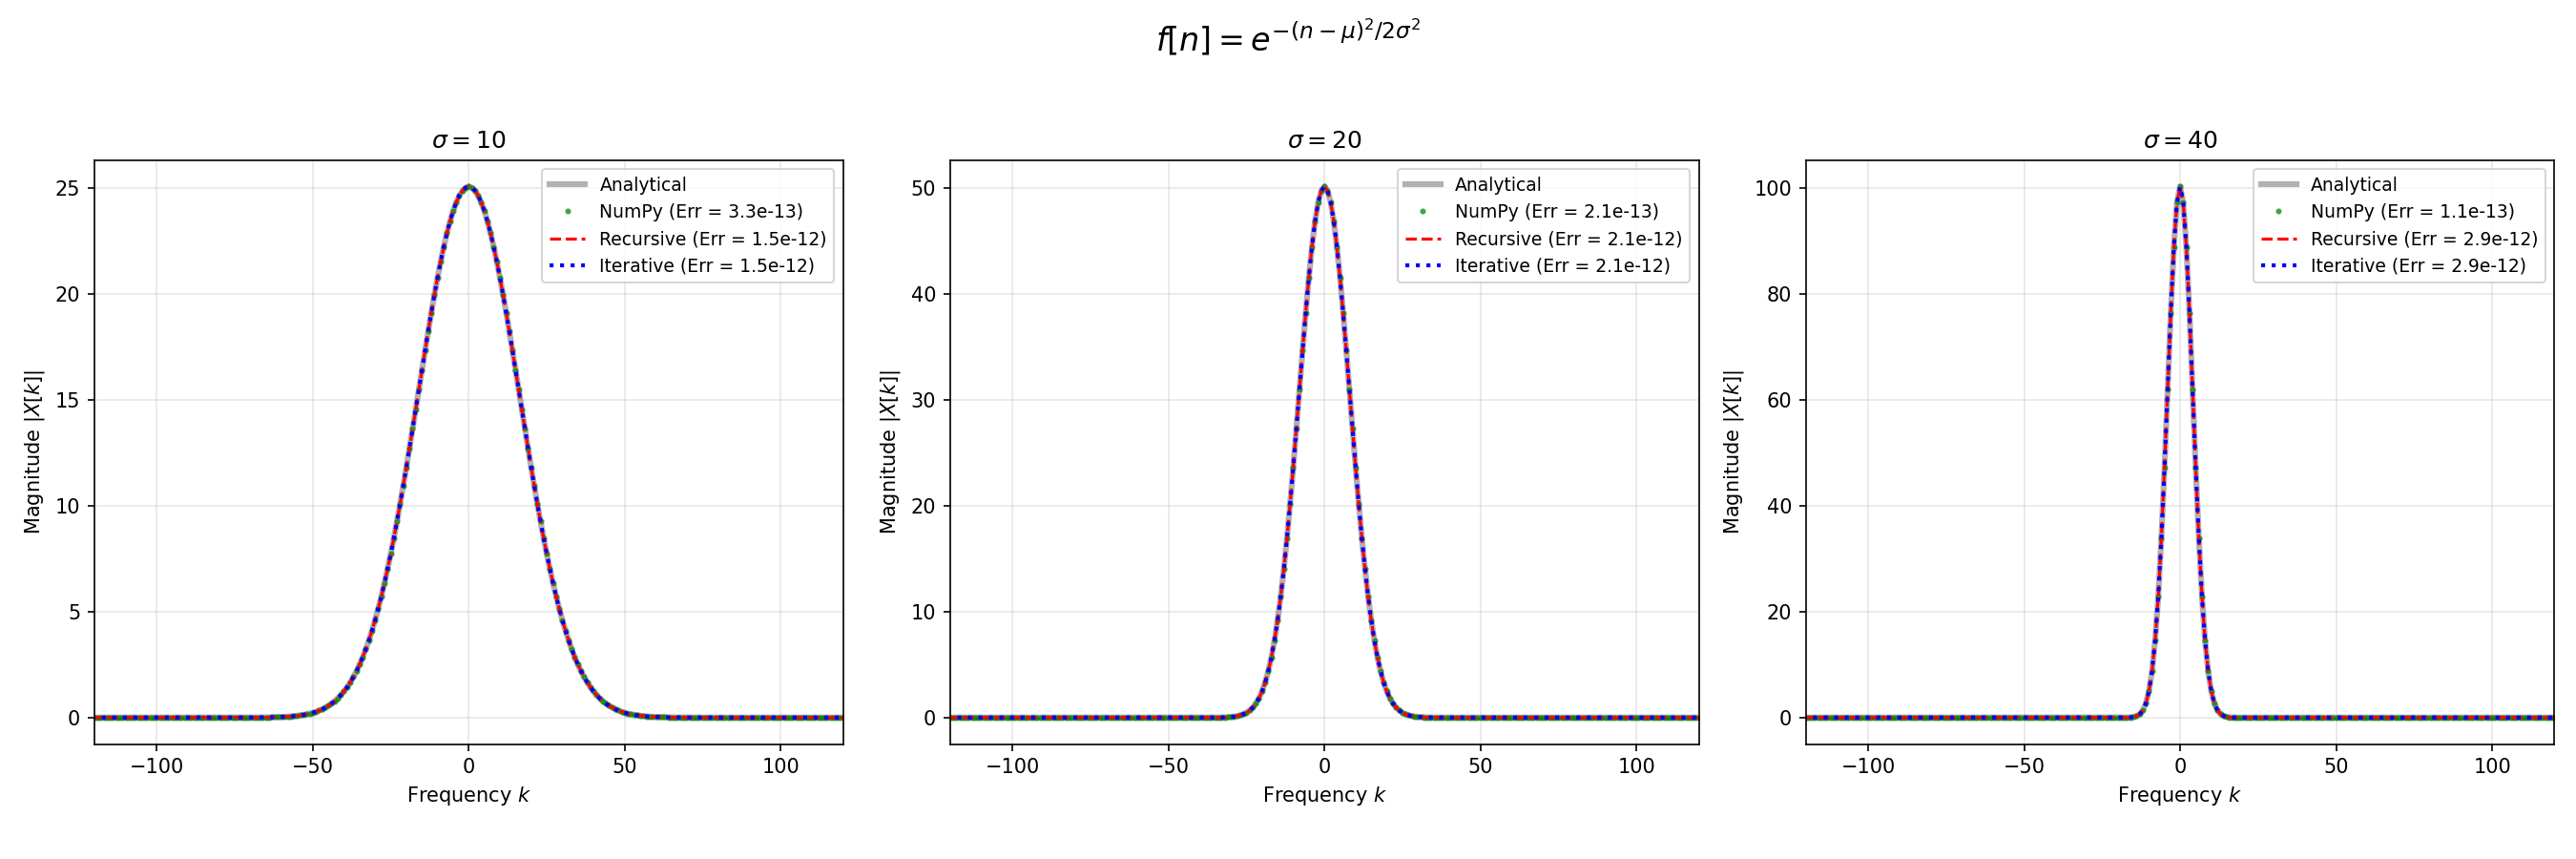
\includegraphics[width=1\linewidth]{../figures/gaussians.png}
    \caption{Comparison between the DFT computed with our recursive and iterative codes, the NumPy routine \texttt{np.fft()}, and the analytical solution for Gaussian signals. $N = 1024$ points are used. The error is the $L^2$ norm.}
    \label{gaussianas}
\end{figure}



\subsection{Kronecker deltas}

\begin{figure}[H]
\centering

\begin{subfigure}{0.8\textwidth}
    \centering
    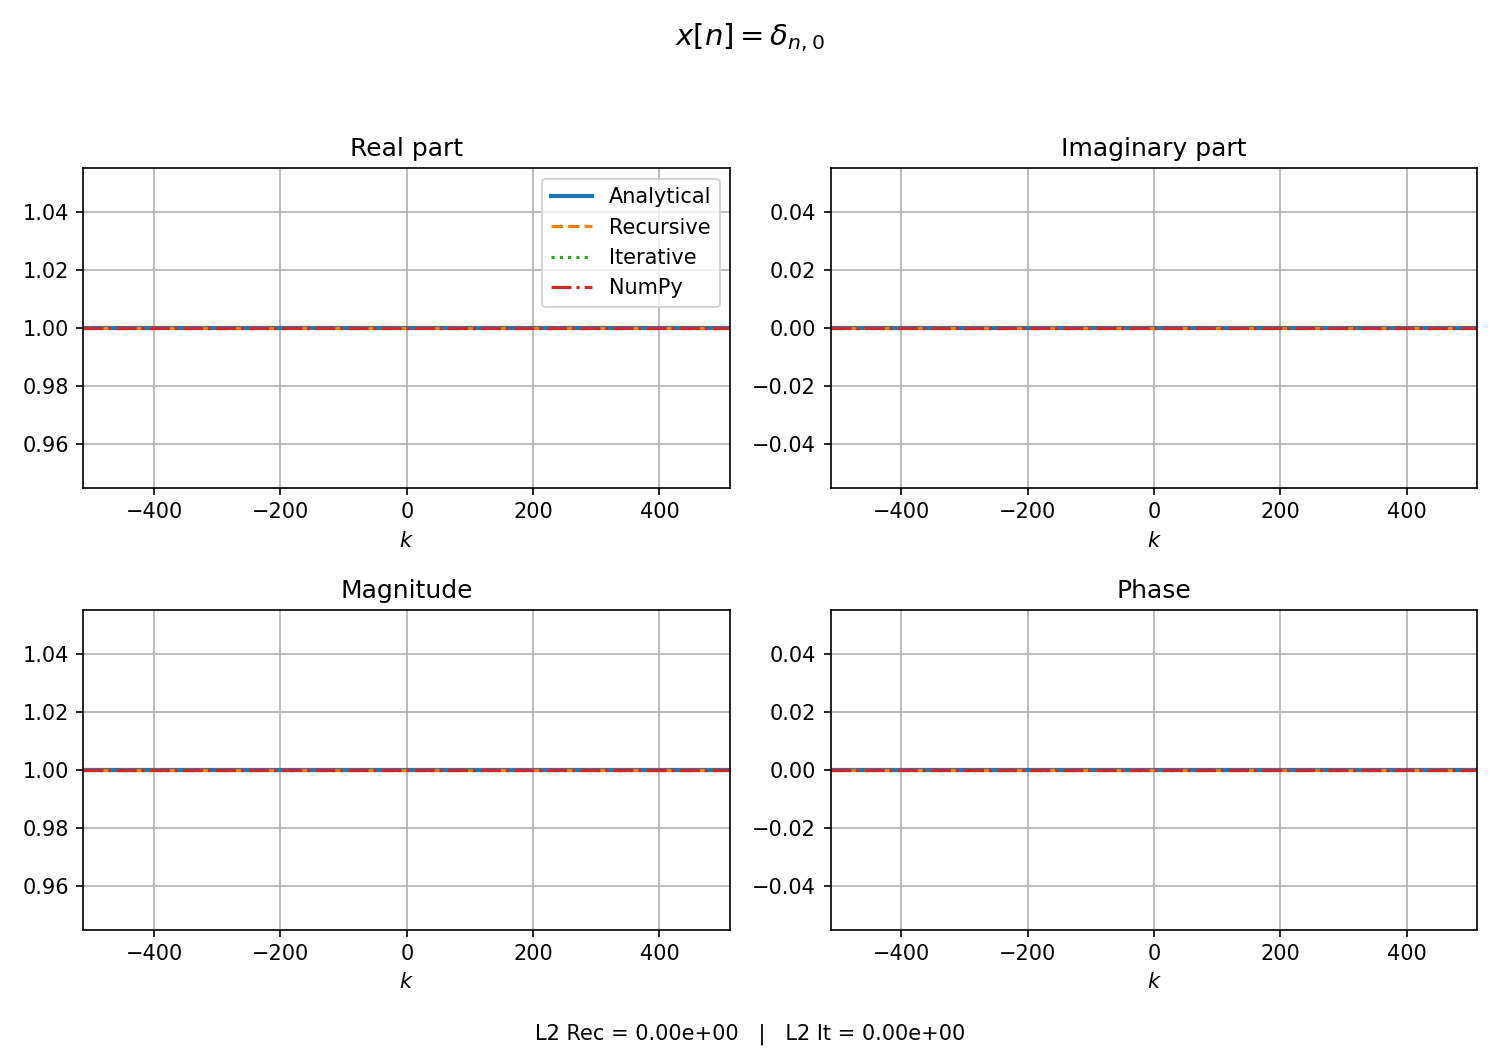
\includegraphics[width=\linewidth]{../figures/delta0.png}
    \caption{$\delta_{n,0}$}
\end{subfigure}

\vfill

\begin{subfigure}{0.8\textwidth}
    \centering
    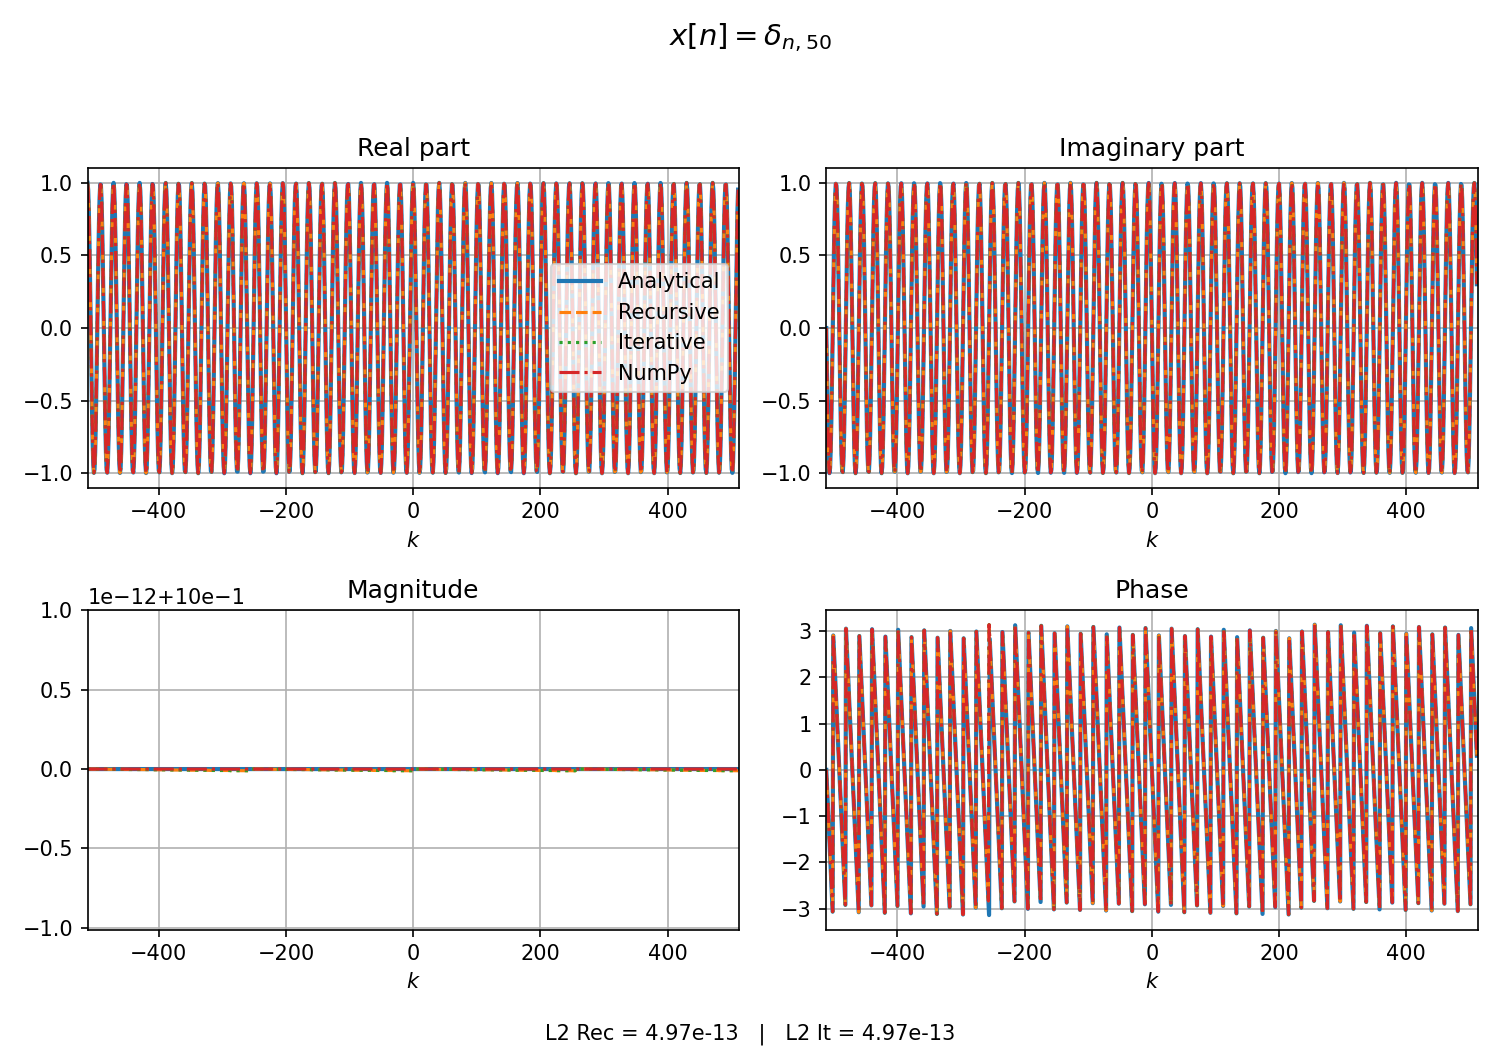
\includegraphics[width=\linewidth]{../figures/delta50.png}
    \caption{$\delta_{n,50}$}
\end{subfigure}

\caption{Comparison between the DFT computed with our recursive and iterative codes, the NumPy routine \texttt{np.fft()}, and the analytical solution for Kronecker delta inputs. $N = 1024$ points are used. The error is the $L^2$ norm.}
\end{figure}



\subsection{Square pulse}

\begin{figure}[H]
    \centering
    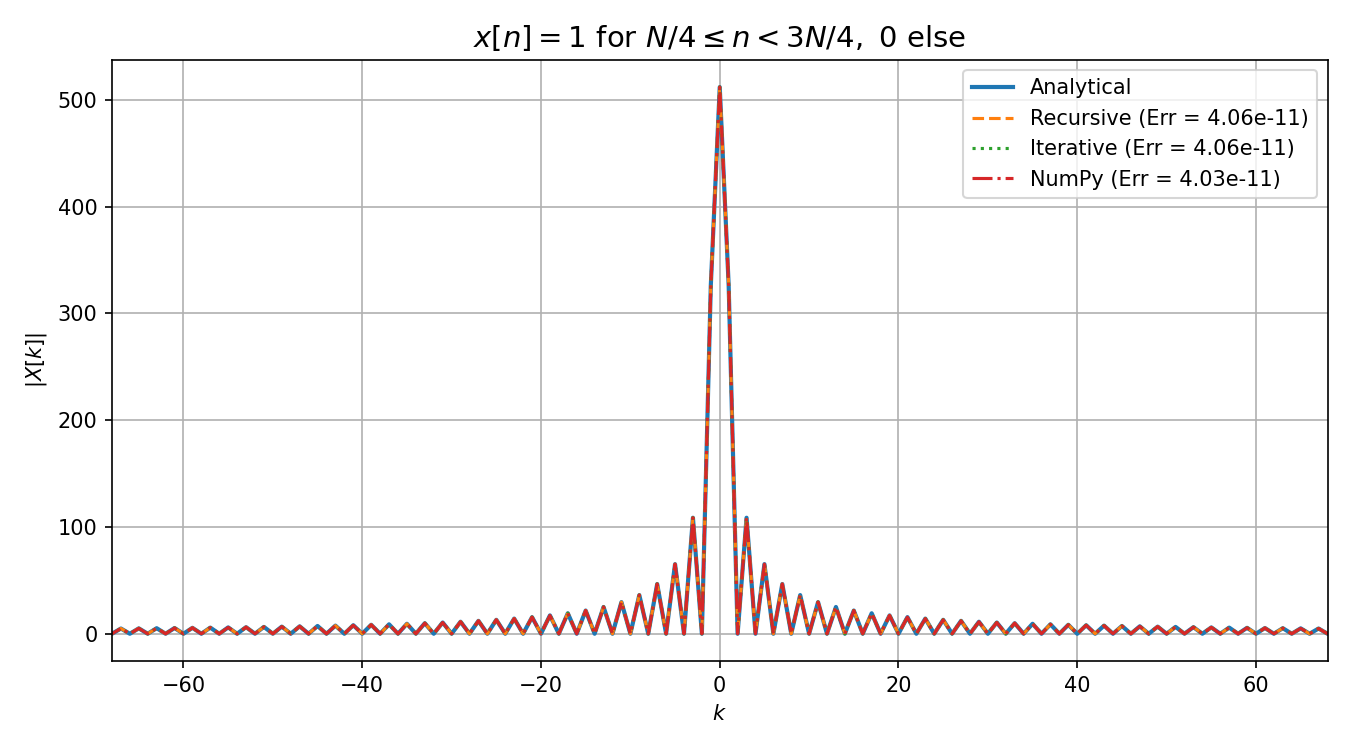
\includegraphics[width=1\linewidth]{../figures/square_pulse.png}
    \caption{Comparison between the DFT computed with our recursive and iterative codes, the NumPy routine \texttt{np.fft()}, and the analytical solution for a square pulse. $N = 1024$ points are used. The error is the $L^2$ norm.}
\end{figure}



\subsection{Constant function}

\begin{figure}[H]
    \centering
    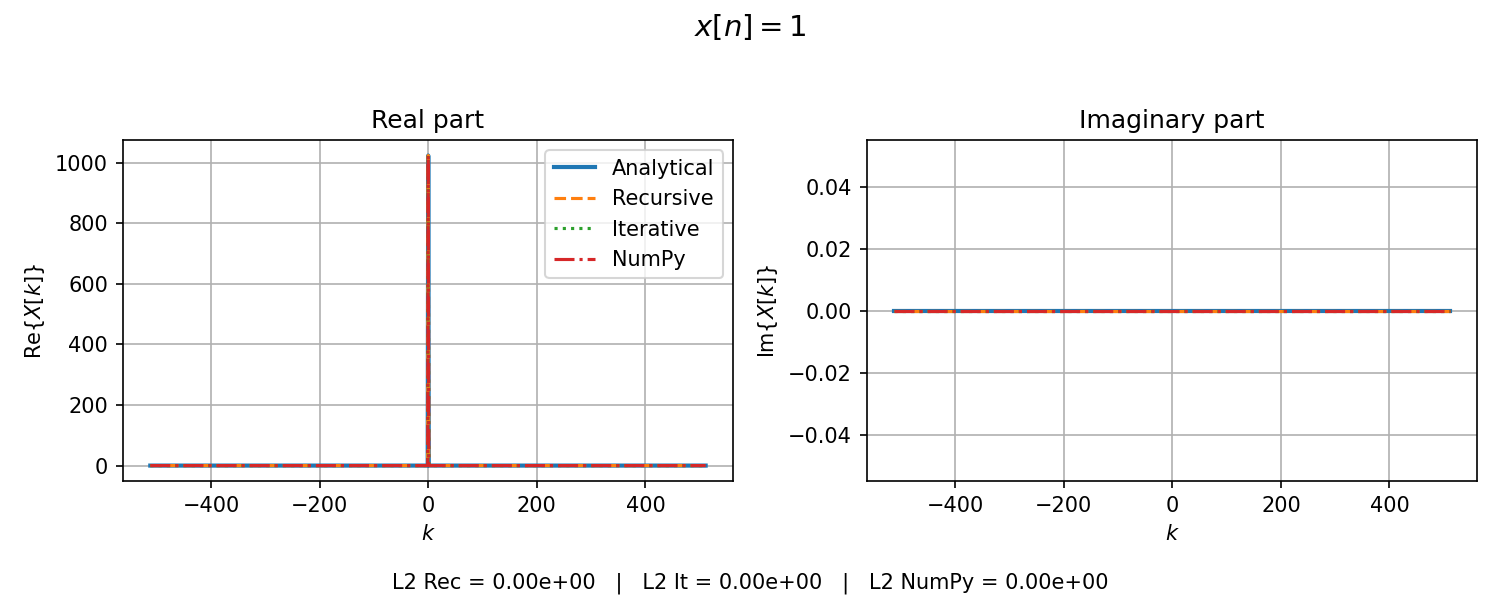
\includegraphics[width=1\linewidth]{../figures/constant.png}
    \caption{Comparison between the DFT computed with our recursive and iterative codes, the NumPy routine \texttt{np.fft()}, and the analytical solution for a constant signal. $N = 1024$ points are used. The error is the $L^2$ norm.}
\end{figure}



\subsection{Plane wave}

\begin{figure}[H]
    \centering
    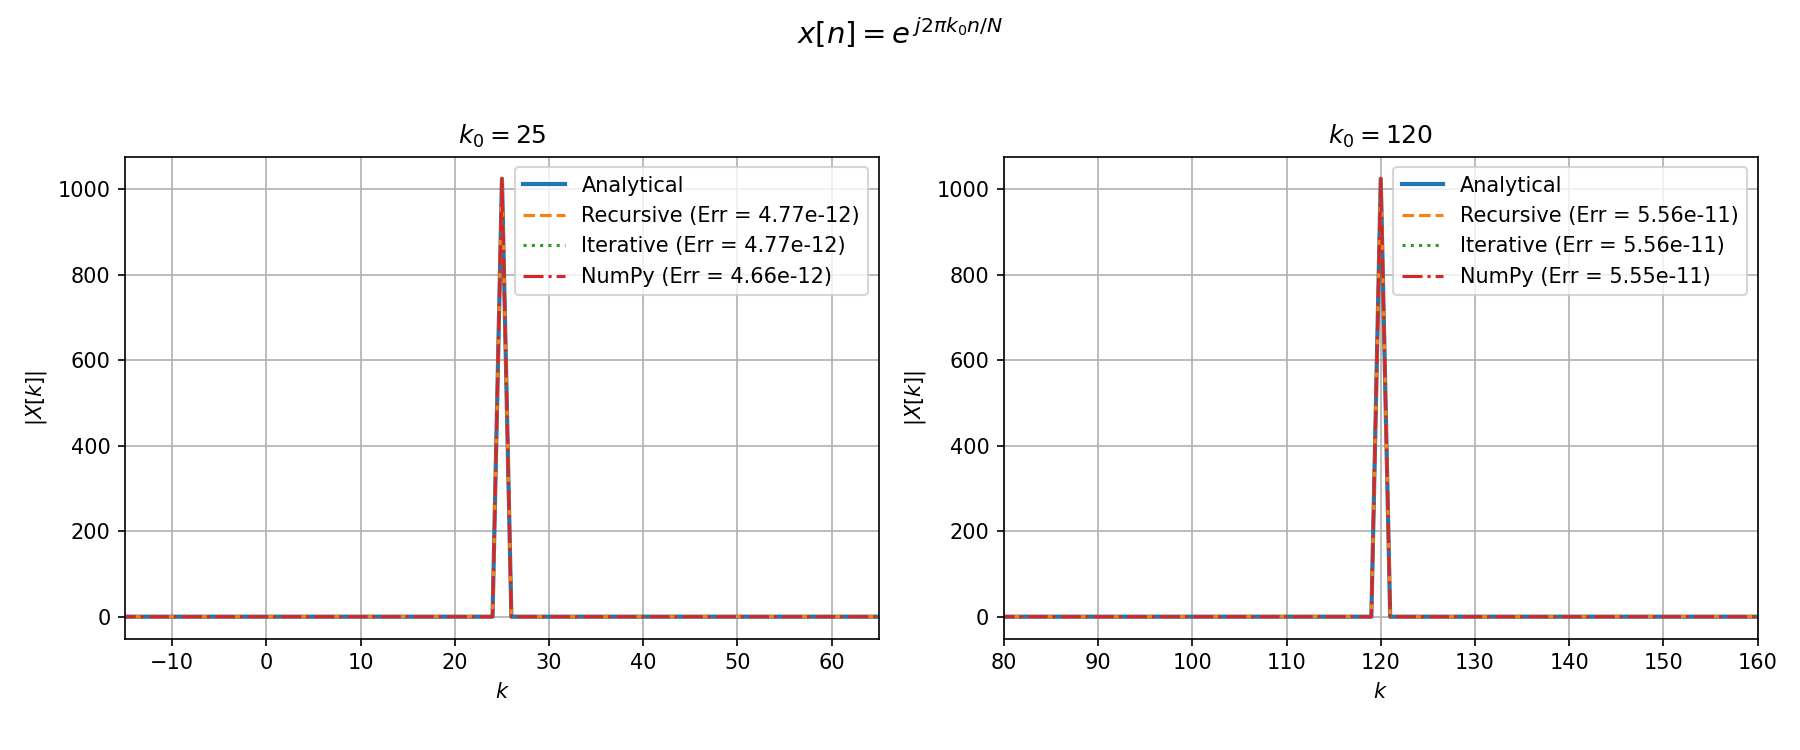
\includegraphics[width=1\linewidth]{../figures/plane_wave.png}
    \caption{Comparison between the DFT computed with our recursive and iterative codes, the NumPy routine \texttt{np.fft()}, and the analytical solution for a complex plane wave $x[n]=e^{j2\pi k_0 n/N}$. $N = 1024$ points are used. The error is the $L^2$ norm.}
\end{figure}




\section{Verification of FFT properties}


The continuous Fourier transform satisfies the following properties

\begin{itemize}
    \item $\mathcal{F}\mathcal{F}^{-1} =\mathcal{F}^{-1}\mathcal{F} = \mathcal{I}$,
    \item $\mathcal{F}^4 = N^2 \, \mathcal{I}$,
    \item Norm conservation (Parseval).
\end{itemize}


The following plot shows the $L^2$ error associated with each property as a function of $N$. Even though the error grows mildly with $N$, it remains of order $10^{-11}$, confirming that the theoretical properties are satisfied by our implementations.


\newpage
\begin{figure}[H]
    \centering
    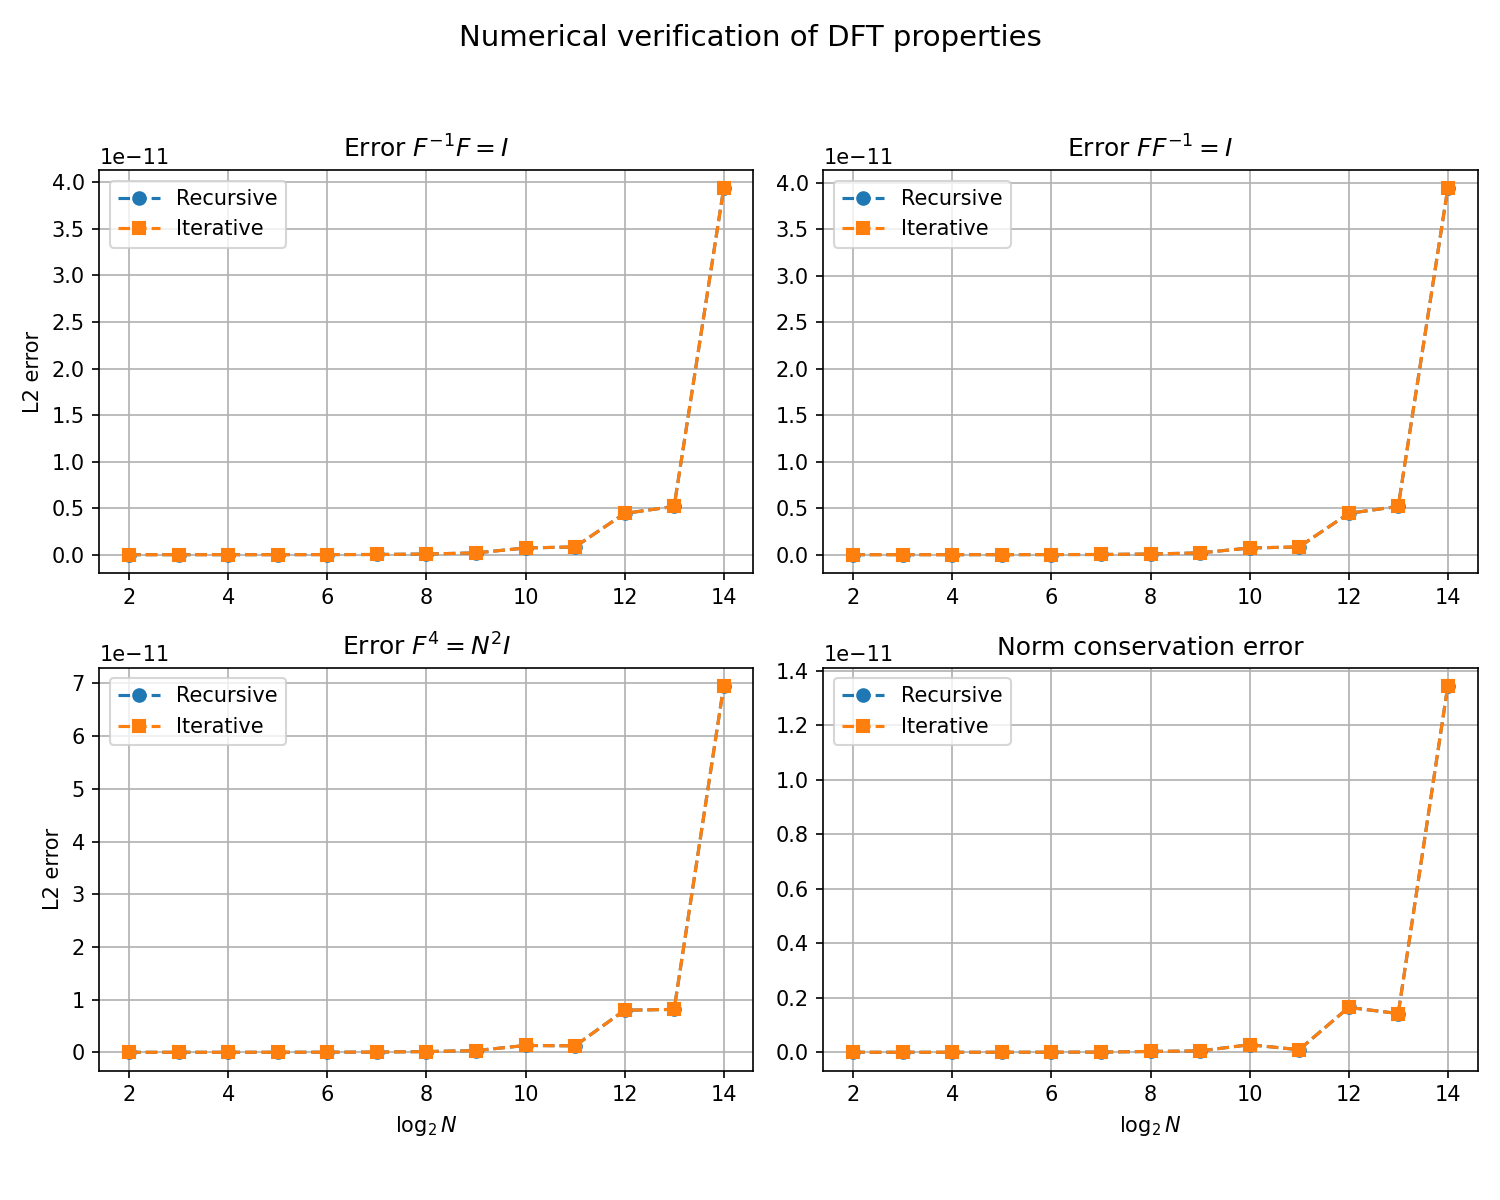
\includegraphics[width=0.8\linewidth]{../figures/properties.png}
    \caption{Verification of the theoretical DFT properties using the codes described in section \ref{intro}. The input is a complex Gaussian random vector with zero mean and unit variance. Results are averaged over $10^2$ realisations. The $x$ axis is in $\log_2 N$ scale. The error is the $L^2$ norm.}
\end{figure}


The last check concerns the execution time, expected to grow as $\mathcal{O}(N\log_2 N)$. As shown in the following plot, normalising by $N\log_2 N$ produces flat curves, confirming the $\mathcal{O}(N\log_2 N)$ scaling. Moreover, no significant difference is observed between the recursive and iterative runtimes.



\begin{figure}[H]
    \centering
    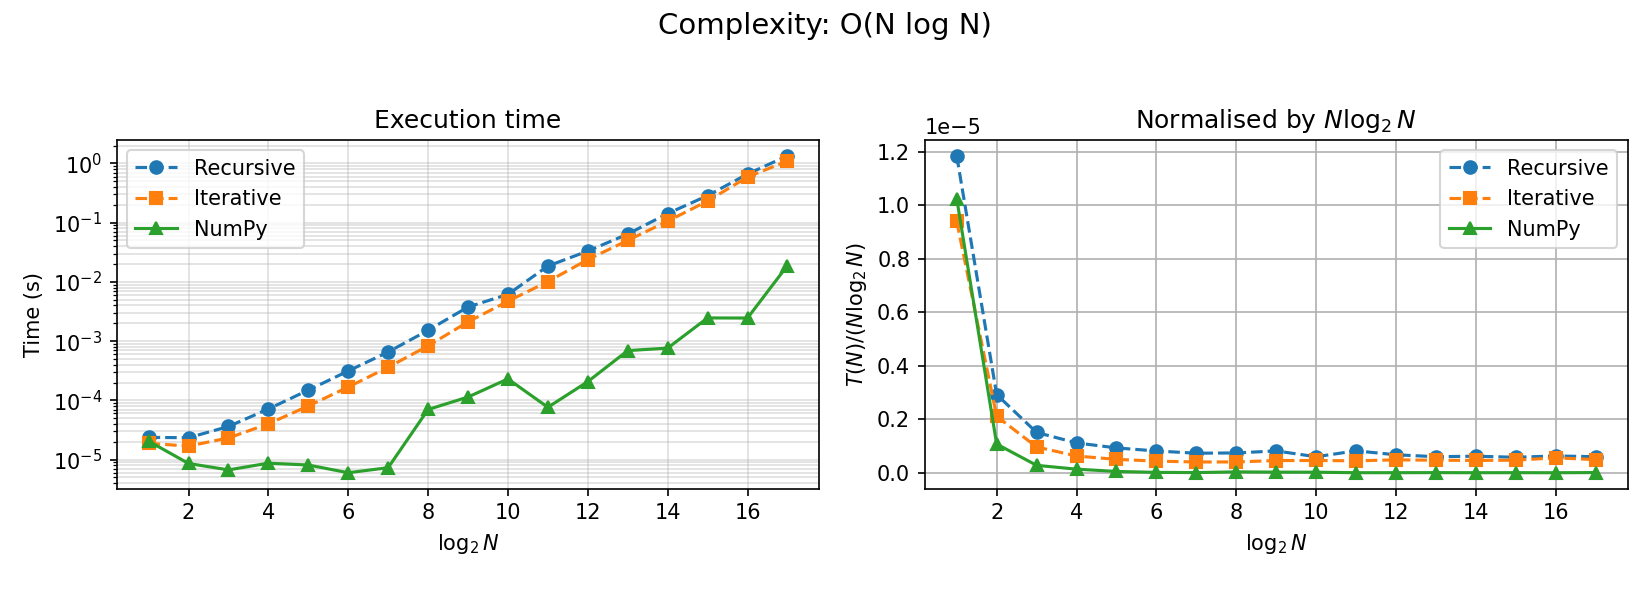
\includegraphics[width=1\linewidth]{../figures/timings.png}
    \caption{Complexity verification for our FFT implementations and \texttt{np.fft()}. The input is a complex Gaussian random vector with zero mean and unit variance.}
\end{figure}




\section{Fourier transform in quantum mechanics}


The wavefunction $\psi$ of a quantum state can be represented both in position space $x$ and in momentum space $p$. The two representations are related by the Fourier transform \cite{sakurai2020modern}

$$
    \phi(p) = \frac{1}{\sqrt{2\pi \hbar}} \int_{-\infty}^{+\infty} \psi(x) e^{-jpx/\hbar} dx,
$$

and its inverse

$$
    \psi(x) = \frac{1}{\sqrt{2\pi \hbar}} \int_{-\infty}^{+\infty} \phi(p) e^{jpx/\hbar} dp.
$$


\subsection{Stationary case}

The time-independent Schr\"odinger equation for a particle in one dimension is

\begin{equation}
\hat H \psi(x) = E \psi(x),
\end{equation}

with Hamiltonian

\begin{equation}
\hat H =
-\frac{\hbar^2}{2m}\frac{d^2}{dx^2}
+ V(x).
\end{equation}

The kinetic operator contains a second derivative, which is expensive to evaluate directly in real space since it couples $x_{n+1}$, $x_{n}$ and $x_{n-1}$. In Fourier space, however,

\begin{equation}
\frac{d^2}{dx^2} \longleftrightarrow -k^2,
\end{equation}

so the kinetic operator becomes diagonal. One can therefore move $\psi(x)$ to momentum space with a Fourier transform, apply the (diagonal) kinetic operator, and come back to real space with an inverse Fourier transform,

\begin{equation}
\hat T
=
\mathcal F^{-1}
\left(
\frac{\hbar^2 k^2}{2m}
\right)
\mathcal F.
\end{equation}


The potential acts in position space as

\begin{equation}
(\hat V\psi)(x)=V(x)\psi(x),
\end{equation}

which is already diagonal. The full discrete Hamiltonian is then

\begin{equation}
H = F^{-1} D F + V.
\end{equation}


\subsection{Time-dependent case}


The formal solution of the time-dependent Schr\"odinger equation is

$$
    \psi(t) = e^{-j\hat{H}t/\hbar} \psi_0.
$$


Since $\hat{T}$ and $\hat{V}$ do not commute, one uses the short-time approximation

$$
    \psi(t + \Delta t) = e^{-j\hat{H}\Delta t/\hbar} \psi(t),
$$


and splits the propagator using the Trotter approximation \cite{kalos2008monte}

$$
    e^{-j\hat{H}\Delta t/\hbar} = e^{-j\hat{T}\Delta t/2\hbar} e^{-j\hat{V}\Delta t/\hbar} e^{-j\hat{T}\Delta t/ 2\hbar} + \mathcal{O} (\Delta t^3).
$$


The resulting algorithm is

\begin{itemize}
    \item [1.] $\psi(x) \to \phi(p)$ via FFT
    \item [2.] multiply by the kinetic phase
    \item [3.] $\phi'(p) \to \psi'(x)$ via IFFT
    \item [4.] multiply by the potential phase
    \item [5.] $\psi''(x) \to \phi''(p)$ via FFT
    \item [6.] multiply by the kinetic phase
    \item [7.] $\phi'''(p) \to \psi'''(x)$ via IFFT
\end{itemize}


\subsection{Example: harmonic oscillator ground state}

As a concrete application we compute the ground-state energy of the one-dimensional quantum harmonic oscillator. In natural units ($\hbar = m = \omega = 1$) the Hamiltonian is

$$
\hat H = -\tfrac{1}{2}\frac{d^2}{dx^2} + \tfrac{1}{2} x^2,
$$

with exact ground-state energy $E_0 = 1/2$ and eigenfunction $\psi_0(x) = \pi^{-1/4} e^{-x^2/2}$.

We use the split-operator method in imaginary time: substituting $t \to -i\tau$ in the evolution operator, the exponential $e^{-\hat H \tau}$ filters out the high-energy components, so any initial state with non-zero overlap with the ground state converges to it. The kinetic operator is applied via FFT as described above.

\begin{figure}[H]
    \centering
    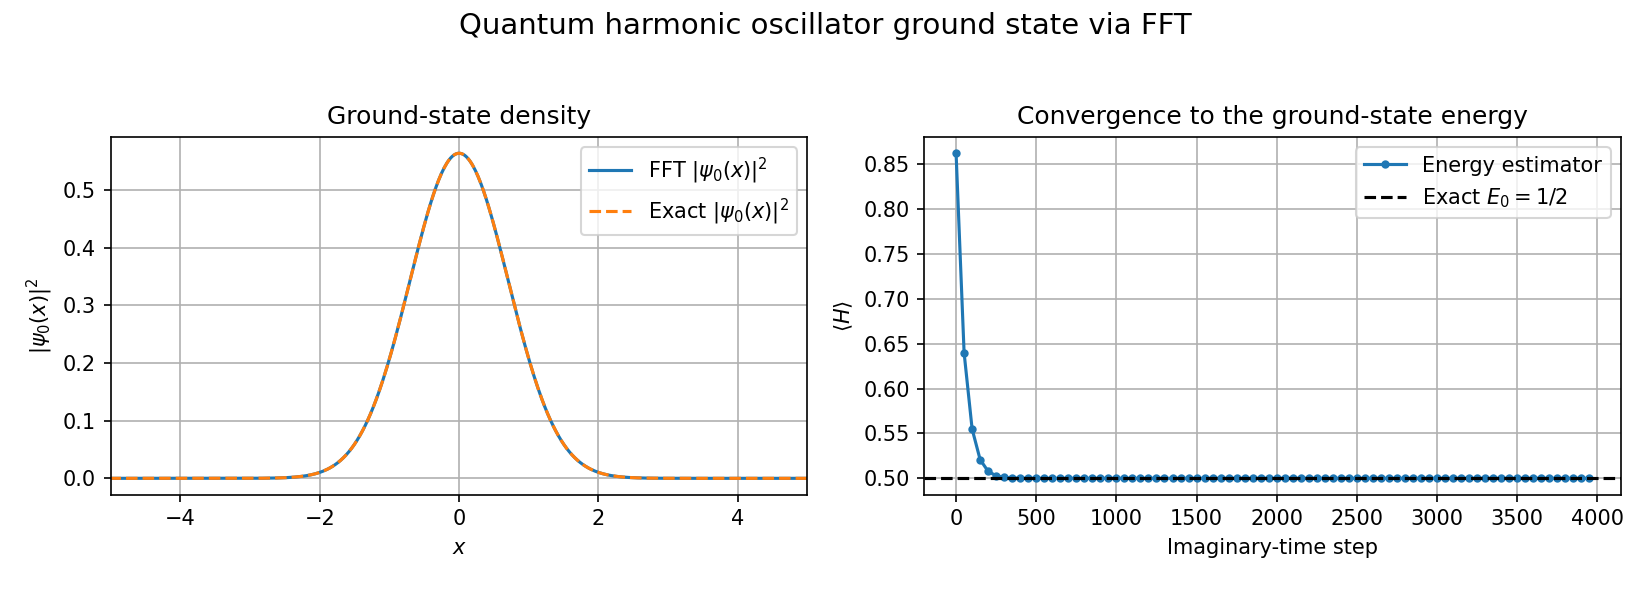
\includegraphics[width=1\linewidth]{../figures/harmonic_oscillator.png}
    \caption{Ground state of the quantum harmonic oscillator obtained by imaginary-time propagation with the FFT-based split-operator method. Left: numerical probability density $|\psi_0(x)|^2$ versus the analytical Gaussian $\pi^{-1/2} e^{-x^2}$. Right: convergence of the energy estimator $\langle H \rangle$ towards the exact value $E_0 = 1/2$.}
\end{figure}



\newpage
\section{Conclusion}



We have studied the discrete Fourier transform and its efficient implementation via the Fast Fourier Transform (FFT), which reduces the original $\mathcal{O}(N^2)$ cost to $\mathcal{O}(N\log_2 N)$ through a recursive decomposition based on the separation of even and odd indices.

Two in-house implementations of the FFT algorithm have been developed, a recursive version and an iterative version based on the \emph{bit-reversal} procedure. Both agree with the NumPy \texttt{np.fft()} routine and with analytical solutions for several representative functions. In all cases, the numerical results show excellent agreement, with errors of order $10^{-10}$.

The implemented algorithms have also been shown numerically to satisfy the fundamental properties of the Fourier transform, namely invertibility, norm conservation and fourth-order periodicity.

The execution-time study confirms that both versions behave consistently with the theoretical $\mathcal{O}(N\log_2 N)$ complexity. Although the iterative version has an advantage in memory usage, no significant runtime difference is observed for the sizes considered.

Finally, the application of the Fourier transform in quantum mechanics has been explored, analysing the relation between position and momentum representations and the numerical solution of the Schr\"odinger equation by spectral methods. The FFT allows an efficient evaluation of the kinetic operator and of the full discrete Hamiltonian, yielding energy levels and eigenfunctions with high precision, as demonstrated here for the quantum harmonic oscillator.



\newpage
\bibliographystyle{plain}
\bibliography{bibliography}




\end{document}
